\section{Edge Coverage and Path Discovery}

This section presents the primary metrics used to evaluate the efficiency of the proposed modifications: total region coverage and queue size. We compare the standard AFL++ baseline with the modified versions across all targets.

\subsubsection{Total Edge Coverage}

The primary indicator of a fuzzer's overall success is the total number of unique code regions discovered over time. To measure this, coverage analysis was performed using \texttt{llvm-cov}. For each campaign, we gathered the inputs saved in the fuzzer's queue and replayed them against an \texttt{llvm-cov}-instrumented binary. By ordering the queue inputs by creation timestamp, we computed the cumulative region coverage over the 24-hour fuzzing campaigns.

The following plots illustrate the average region coverage growth for each benchmark over 24 hours.

% --- PAGE 1 ---
\begin{figure}[htbp]
    \centering

    \begin{subfigure}{\textwidth}
        \centering
        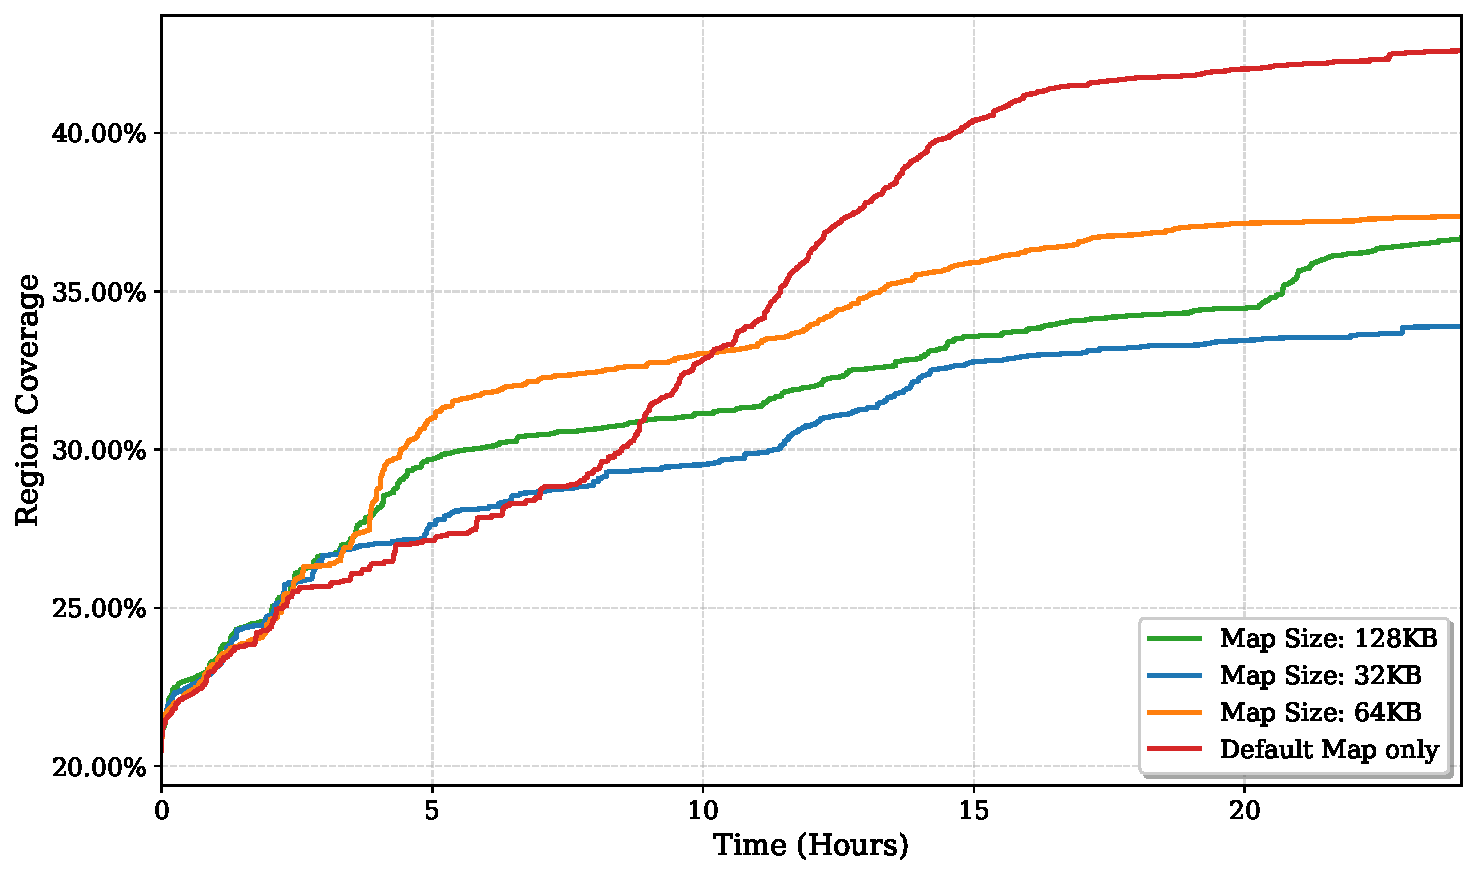
\includegraphics[width=0.85\linewidth]{imgs/eval/coverage_plot_mruby.pdf}
        \caption{mruby}
        \label{fig:plot_mruby}
    \end{subfigure}

    \vspace{2em} 

    \begin{subfigure}{\textwidth}
        \centering
        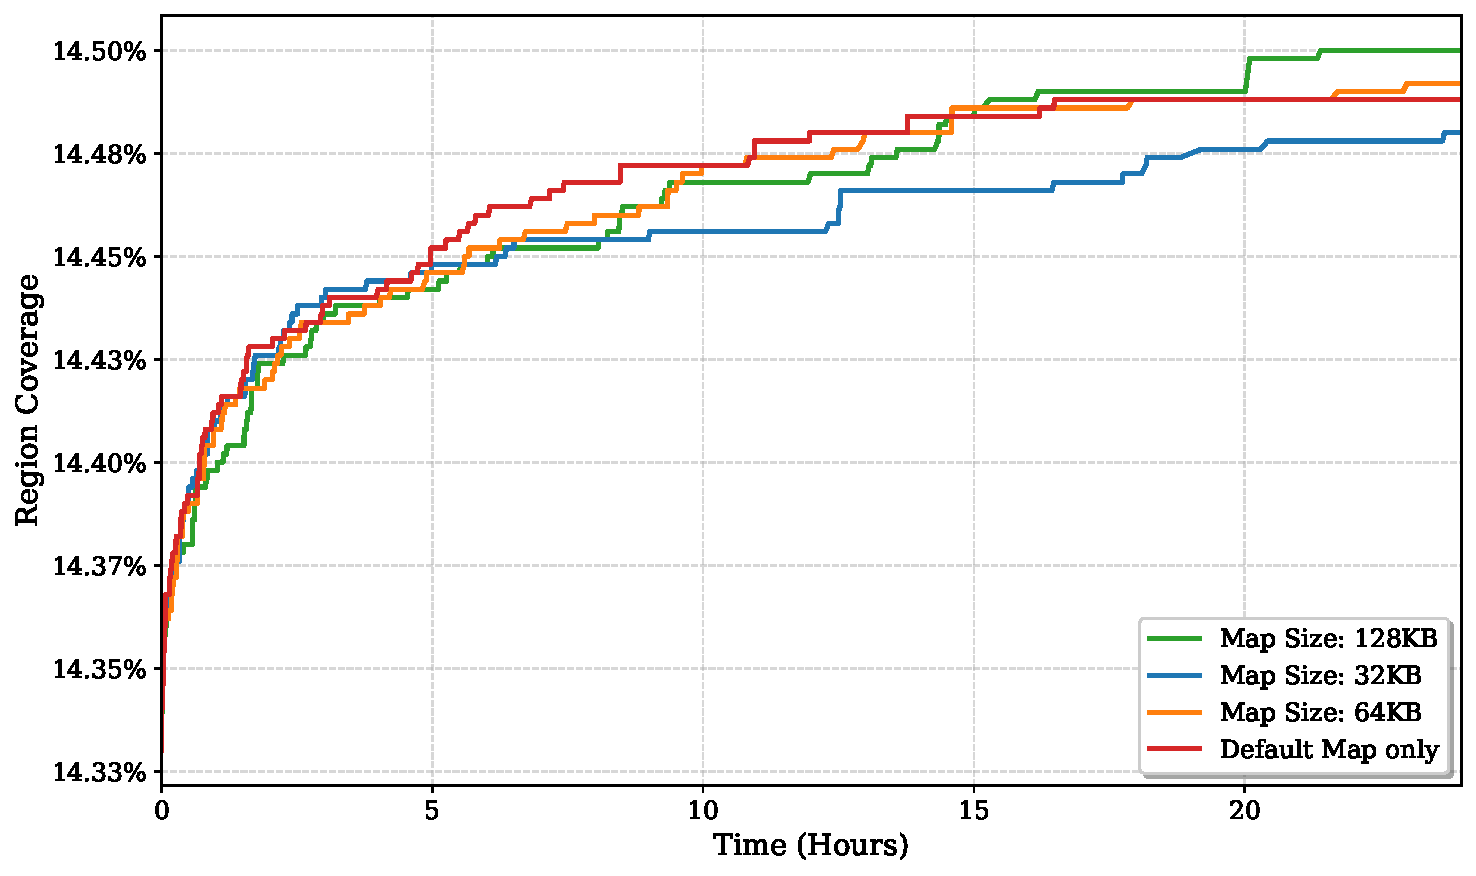
\includegraphics[width=0.85\linewidth]{imgs/eval/coverage_plot_openssl.pdf}
        \caption{OpenSSL}
        \label{fig:plot_openssl}
    \end{subfigure}

    \caption{Coverage over 24 hours for various fuzzing targets (Part 1).}
\end{figure}

% --- PAGE 2 OF THE FIGURE ---
\begin{figure}[htbp]
    \ContinuedFloat % This keeps the figure number the same
    \centering

    \begin{subfigure}{\textwidth}
        \centering
        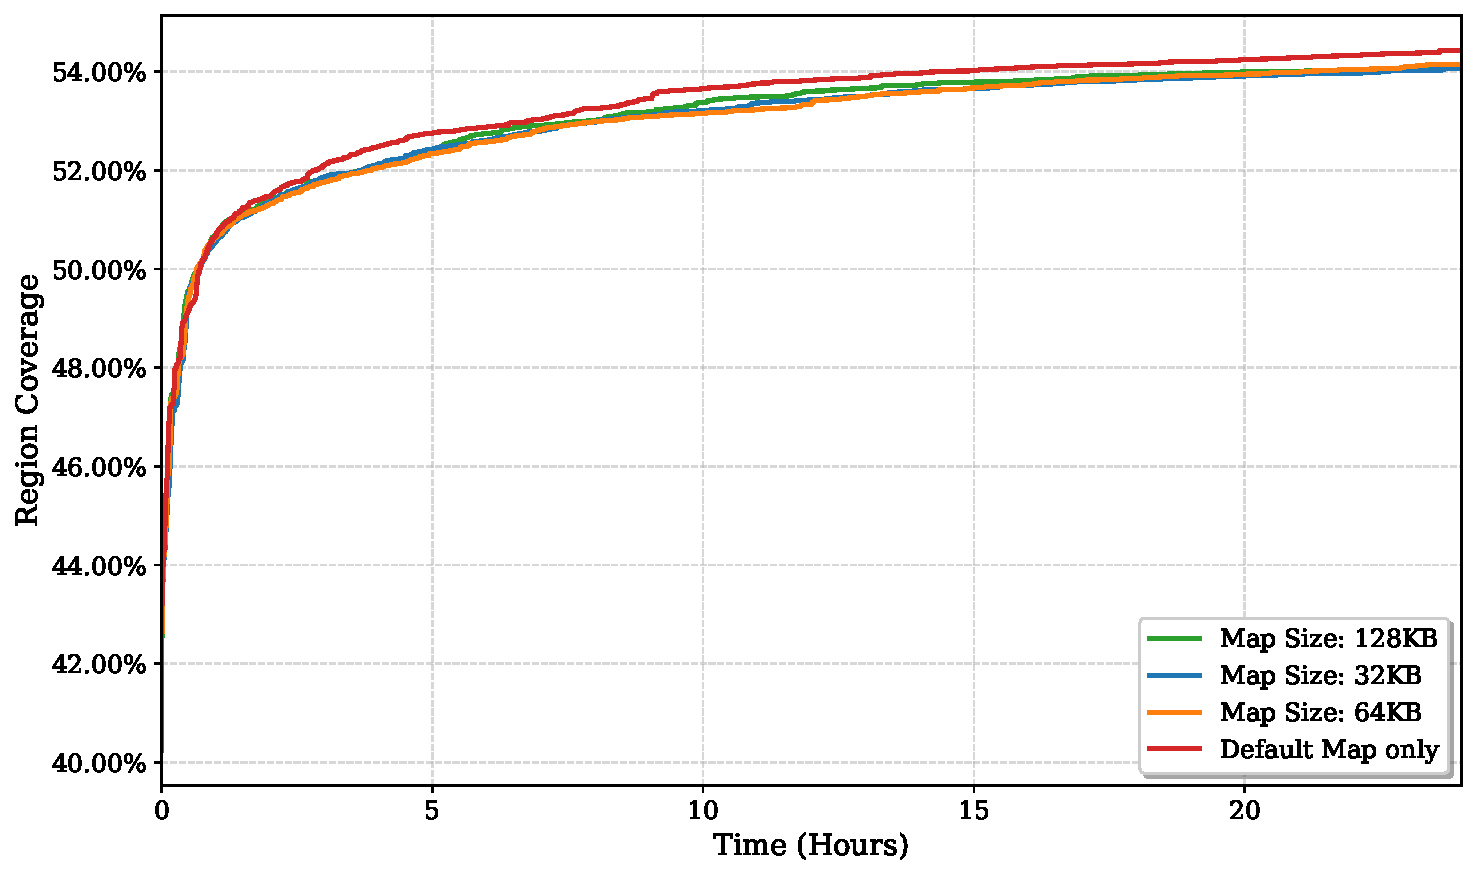
\includegraphics[width=0.85\linewidth]{imgs/eval/coverage_plot_libxslt.pdf}
        \caption{libxslt}
        \label{fig:plot_libxslt}
    \end{subfigure}
    
    \vspace{2em}

    \begin{subfigure}{\textwidth}
        \centering
        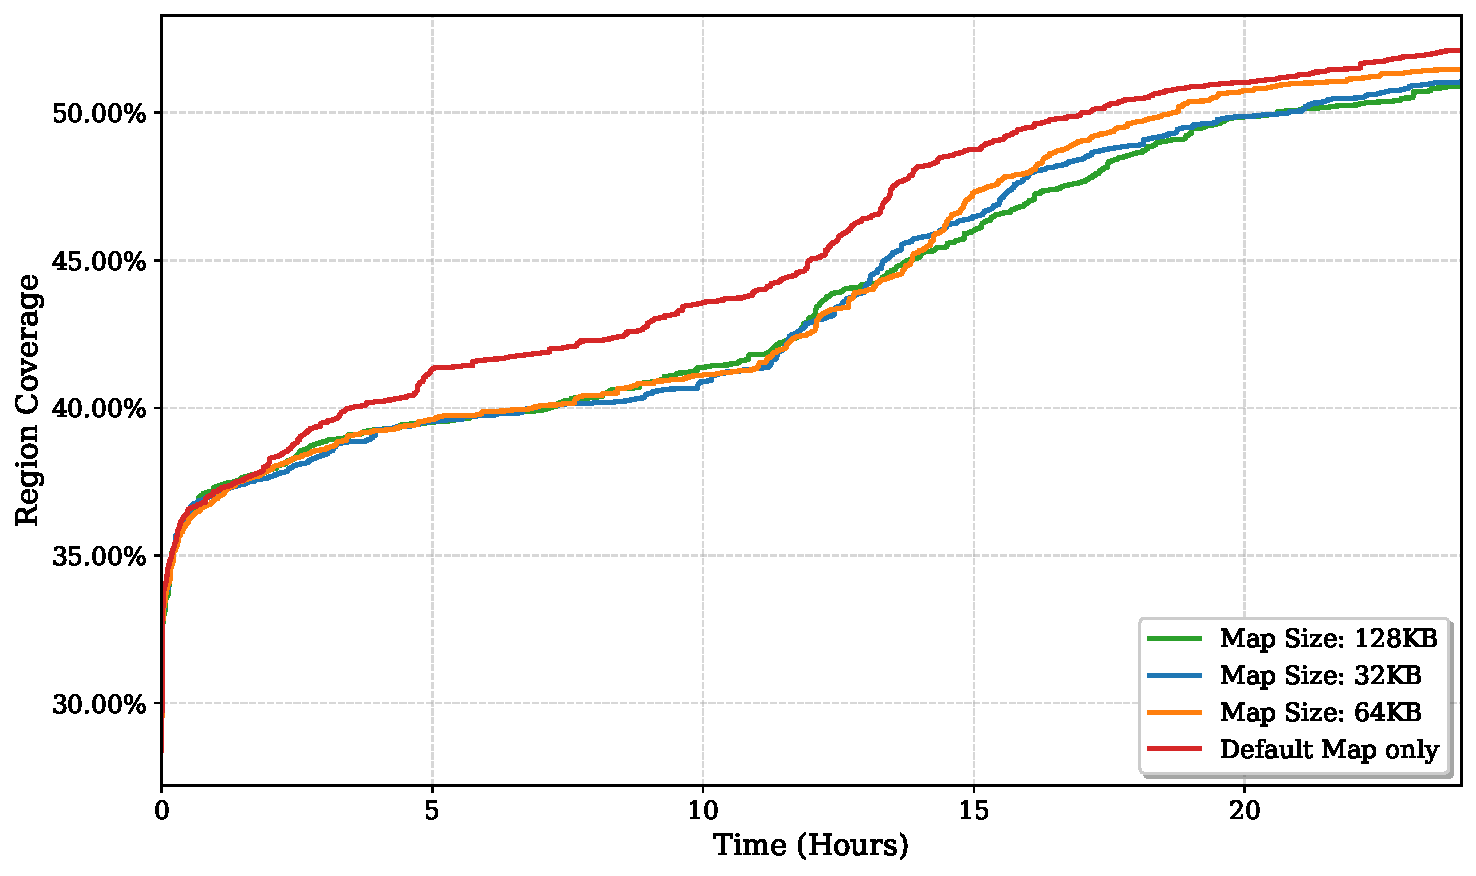
\includegraphics[width=0.85\linewidth]{imgs/eval/coverage_plot_sqlite3.pdf}
        \caption{SQLite3}
        \label{fig:plot_sqlite3}
    \end{subfigure}
    
    \caption{Coverage over 24 hours for various fuzzing targets (Part 2).}
\end{figure}


\begin{figure}[htbp]
    \ContinuedFloat % This keeps the figure number the same
    \centering

    \begin{subfigure}{\textwidth}
        \centering
        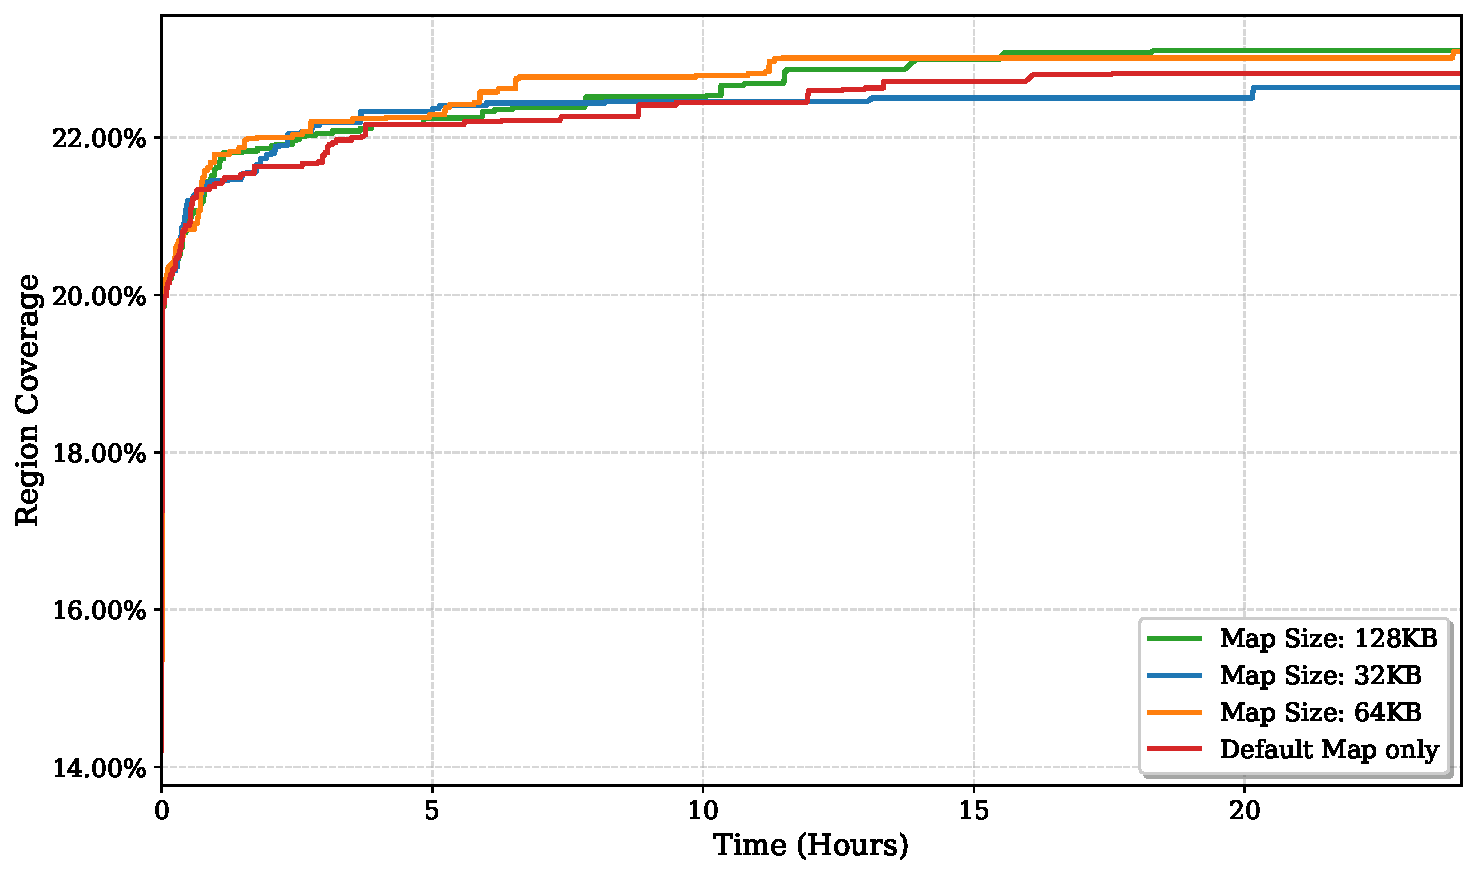
\includegraphics[width=0.85\linewidth]{imgs/eval/coverage_plot_systemd.pdf}
        \caption{systemd}
        \label{fig:plot_systemd}
    \end{subfigure}

    \caption{Coverage over 24 hours for various fuzzing targets (Part 3).}
    \label{fig:cov_plots} % The main label 
\end{figure}

\newpage

The results reveal that, across all tested benchmarks, the modified fuzzer configurations did not achieve a breakthrough in path discovery. In fact, the baseline AFL++ consistently performed either on par with or slightly better than the modified versions in terms of discovered regions within the given time frame.

Table \ref{tab:region_coverage} shows the cumulative region coverage at the end of the campaign for each target and configuration.

\begin{table}[htbp]
    \centering
    \begin{tabular}{@{}l cccc @{}}
        \toprule
        & \multicolumn{4}{c}{\textbf{Fuzzer Configuration}} \\
        \cmidrule(l){2-5}
        \textbf{Target} & \textbf{32 bit} & \textbf{64 bit} & \textbf{128 bit} & \textbf{Default} \\
        \midrule
        \textbf{libxslt} & 54.06\% & 54.14\% & 54.06\% & 54.43\% \\
        \textbf{mruby}   & 33.89\% & 37.36\% & 36.70\% & 42.61\% \\
        \textbf{openssl} & 14.48\% & 14.49\% & 14.50\% & 14.48\% \\
        \textbf{sqlite3} & 51.04\% & 51.46\% & 50.88\% & 52.11\% \\
        \textbf{systemd} & 23.10\% & 23.57\% & 23.58\% & 23.29\% \\
        \bottomrule
    \end{tabular}
    \caption{Average Region Coverage after 24 Hours}
    \label{tab:region_coverage}
\end{table}

Variations across configurations are generally minor. The 32-bit configuration more consistently results in the lowest region coverage among the modified setups. This can be attributed to a higher probability of collisions within the smaller Bloom filter, which saturates prematurely. The 64-bit and 128-bit configurations performed marginally better; however, they consistently failed to outperform the vanilla AFL++ baseline.

\subsubsection{Corpus Size}

The fuzzer's corpus (or queue) size indicates the number of unique "interesting" test cases retained during the campaign. A steadily growing queue typically indicates the continuous discovery of new paths.

The final queue sizes at the end of the campaigns are summarised in Table \ref{tab:corpus_sizes}.

\begin{table}[htbp]
\centering
\begin{tabular}{lrrrr}
\toprule
& \multicolumn{4}{c}{\textbf{Fuzzer Configuration}} \\
\cmidrule(l){2-5}
\textbf{Target} & \textbf{32 bit} & \textbf{64 bit} & \textbf{128 bit} & \textbf{Default} \\
\midrule
\textbf{libxslt} & 17,509.20 & 17,751.60 & 17,504.60 & 18,127.00 \\
\textbf{mruby}   & 5,881.40  & 8,414.80  & 7,381.00  & 11,122.80 \\
\textbf{openssl} & 2,909.20  & 2,916.40  & 2,935.80  & 2,931.00 \\
\textbf{sqlite3} & 11,054.40 & 10,761.80 & 9,875.80  & 13,026.00 \\
\textbf{systemd} & 2,173.40  & 2,125.80  & 2,171.00  & 2,261.00 \\
\bottomrule
\end{tabular}
\caption{Average Corpus Sizes after 24 Hours}
\label{tab:corpus_sizes}
\end{table}

The queue size dynamics closely mirror the region coverage data. Across all targets, the baseline AFL++ and the modified configurations maintain similar queue sizes.

This strongly implies that the indirect map rarely triggered additional seed saves. When an indirect branch was resolved dynamically, the input was almost always already flagged as "interesting" by the primary coverage map.